\documentclass[UTF8,titlepage]{article}
\usepackage{amsmath,amssymb,amsthm,amsfonts,amscd}
\usepackage{fontspec}
\setmainfont{Times New Roman}
\usepackage{graphicx}
\usepackage{titlesec}
\usepackage{makecell}
\usepackage{longtable}
\usepackage{xcolor}
\usepackage{tcolorbox}
\usepackage{soul}
\usepackage{adjustbox}
\usepackage{tcolorbox}
\usepackage{enumerate}
\usepackage{pdfpages}
\usepackage{float}
\usepackage{colortbl}
\usepackage{tabularx}
\usepackage{multirow}
\usepackage{pgfplots}
\numberwithin{figure}{section}
\usepackage[left=1.25in,right=1.25in,%
top=1in,bottom=1in]{geometry}
\usepackage{color}
\titleformat{\section}
  {\raggedright\LARGE\bfseries}{\thesection}{1em}{}
\title{Answer for Problem Set 1}
\author{Boyuan Zhao}
\begin{document}
\begin{center}
    {\LARGE \textbf{Answer of Problem Set 4}}\\  % 这就是你的标题
    {\normalsize Boyuan Zhao}\\  % 这就是你的名字
    {\small \today}  % 这是日期
\end{center}
\section{Problem 1. Production: cost minimization and profit maximization.}
\begin{enumerate}
    \item 1. The cost minimization problem is given by:

    \[\min _{L, K, F} w L+r K+s F\]
    
    subject to the constraint:
    
    \[y=f(L, K, F)\]
    
    The Lagrangian for this problem is:
    
    \[\mathcal{L}=w L+r K+s F+\lambda(y-f(L, K, F))\]
    
    The first order conditions are:
    
    \begin{align*}
    \frac{\partial \mathcal{L}}{\partial L}=w-\lambda f_{L}=0 \\
    \frac{\partial \mathcal{L}}{\partial K}=r-\lambda f_{K}=0 \\
    \frac{\partial \mathcal{L}}{\partial F}=s-\lambda f_{F}=0
    \end{align*}
    \item The cost function is given by:

    \[c(w, r, s, y)=w L^{*}(w, r, s, y)+r K^{*}(w, r, s, y)+s F^{*}(w, r, s, y)\]
    
    The firm maximizes  p y-c(w, r, s, y) . The first order condition with respect to  y  is:
    
    \[\frac{\partial(p y-c(w, r, s, y))}{\partial y}=p-\frac{\partial c(w, r, s, y)}{\partial y}=0\]
    
    \item The profit maximization problem is given by:

    \[\max _{L, K, F} p y-w L-r K-s F\]
    
    The first order conditions are:
    
    \begin{align*}
        \frac{\partial \pi}{\partial L}=p f_{L}-w=0 \\
        \frac{\partial \pi}{\partial K}=p f_{K}-r=0 \\
        \frac{\partial \pi}{\partial F}=p f_{F}-s=0 \\
    \end{align*}
    \item By the envelope theorem, we have:

    \[\frac{\partial c(w, r, s, y)}{\partial y}=\lambda \]
    
    Comparing the first order conditions from the cost minimization and profit maximization problems, we can see that they are equivalent if we set  $\lambda=p$ . This shows that the cost minimization and profit maximization problems are equivalent.
                   
\end{enumerate}

\clearpage

\section{Problem 2. Production: perfect competition.}

\begin{enumerate}
    \item The cost minimization problem is given by:

    \begin{align*}
        \min _{L, K} & w L+r K+s \bar{F} \\
        \text { s.t. } & y=A L^{\alpha} K^{\beta} \bar{F}^{\gamma}
    \end{align*}
    
    The Lagrangian for this problem is:
    
    \[\mathcal{L}=w L+r K+s \bar{F}-\lambda\left(A L^{\alpha} K^{\beta} \bar{F}^{\gamma}-y\right)\]
    
    The first order conditions are given by taking the derivative of the Lagrangian with respect to  $L, K$ , and  $\lambda$ , and setting them equal to zero:
    
    \begin{align*}
        \frac{\partial \mathcal{L}}{\partial L}=w-\lambda \alpha A L^{\alpha-1} K^{\beta} \bar{F}^{\gamma}=0 \\
        \frac{\partial \mathcal{L}}{\partial K}=r-\lambda \beta A L^{\alpha} K^{\beta-1} \bar{F}^{\gamma}=0 \\
        \frac{\partial \mathcal{L}}{\partial \lambda}=A L^{\alpha} K^{\beta} \bar{F}^{\gamma}-y=0
    \end{align*}
    
    \item Given the first order conditions from the Lagrangian:
    \begin{align*}
    \frac{\partial \mathcal{L}}{\partial L} &= w-\lambda \alpha A L^{\alpha-1} K^{\beta} \bar{F}^{\gamma}=0 \\
    \frac{\partial \mathcal{L}}{\partial K} &= r-\lambda \beta A L^{\alpha} K^{\beta-1} \bar{F}^{\gamma}=0
    \end{align*}
    
    We can solve these two equations to find the optimal values of \( L \) and \( K \), denoted \( L^{*} \) and \( K^{*} \).
    First, divide the first equation by the second:
    
    \[
    \frac{w-\lambda \alpha A L^{\alpha-1} K^{\beta} \bar{F}^{\gamma}}{r-\lambda \beta A L^{\alpha} K^{\beta-1} \bar{F}^{\gamma}}=\frac{w}{r} \frac{\beta}{\alpha}
    \]
    
    This simplifies to:
    
    \[
    \frac{K}{L}=\frac{w \beta}{r \alpha}
    \]
    
    Substitute this into the constraint \( A L^{\alpha} K^{\beta} \bar{F}^{\gamma}=y \), we get:
    
    \[
    A L^{\alpha}\left(\frac{w \beta}{r \alpha} L\right)^{\beta} \bar{F}^{\gamma}=y
    \]
    
    Solving for \( L \), we get:
    
    \[
    L^{*}=\left(\frac{y}{A\bar{F}^{\gamma}}\right)^{\frac{1}{\alpha+\beta}}\left(\frac{w \beta}{r \alpha}\right)^{-\frac{\beta}{\alpha+\beta}}
    \]
    
    Substitute \( L^{*} \) into the equation \( \frac{K}{L}=\frac{w \beta}{r \alpha} \), we can solve for \( K^{*} \):
    
    \[
    K^{*}=\left(\frac{y}{A\bar{F}^{\gamma}}\right)^{\frac{1}{\alpha+\beta}}\left(\frac{w \beta}{r \alpha}\right)^{\frac{\alpha}{\alpha+\beta}}
    \]
    \item Given the expression for \( L^{*} \) :

\[
L^{*}=\left(\frac{y}{A\bar{F}^{\gamma}}\right)^{\frac{1}{\alpha+\beta}}\left(\frac{w \beta}{r \alpha}\right)^{-\frac{\beta}{\alpha+\beta}}
\]

We can compute the partial derivative of \( L^{*} \) with respect to \( w \) :

\begin{align*}
\frac{\partial L^{*}}{\partial w} & =\left(\frac{y}{A\bar{F}^{\gamma}}\right)^{\frac{1}{\alpha+\beta}}\left(-\frac{\beta}{\alpha+\beta}\right)\left(\frac{\beta}{r \alpha}\right)\left(\frac{w \beta}{r \alpha}\right)^{-\frac{\beta}{\alpha+\beta}-1} \\
& =-\frac{\beta}{\alpha+\beta}\left(\frac{y}{A\bar{F}^{\gamma}}\right)^{\frac{1}{\alpha+\beta}}\left(\frac{\beta}{r \alpha}\right)\left(\frac{w \beta}{r \alpha}\right)^{-\frac{\alpha+\beta}{\alpha+\beta}}
\end{align*}

Since \( \beta>0 \) and \( \alpha+\beta>0 \), the sign of \( \frac{\partial L^{*}}{\partial w} \) depends on the value of \( w \). If \( w \) is positive, then \( \frac{\partial L^{*}}{\partial w}<0 \), meaning that an increase in the wage rate leads to a decrease in the optimal amount of labor. 

Now considering what happens if there is technological progress and \( A \) increases. We can compute the partial derivative of \( L^{*} \) with respect to \( A \) :

\[
\frac{\partial L^{*}}{\partial A}=-\frac{1}{\alpha+\beta}\left(\frac{y}{A\bar{F}^{\gamma}}\right)^{\frac{1}{\alpha+\beta}-1}\left(\frac{w \beta}{r \alpha}\right)^{-\frac{\beta}{\alpha+\beta}}\left(\frac{1}{A\bar{F}^{\gamma}}\right)
\]

Since \( \alpha+\beta>0 \), the sign of \( \frac{\partial L^{*}}{\partial A} \) depends on the value of \( A \). If \( A \) is positive, then \( \frac{\partial L^{*}}{\partial A}<0 \), meaning that an increase in the technological parameter \( A \) leads to a decrease in the optimal amount of labor. 

\item The cost function \(c(w, r, s, y, \bar{F})\) is given by the minimum cost of producing a given output level \(y\), given the input prices \(w\), \(r\), and \(s\), and the fixed amount of land \(\bar{F}\). 

Using the optimal values of \(L^{*}\) and \(K^{*}\) we derived earlier, we can write the cost function as:

$$
c(w, r, s, y, \bar{F}) = wL^{*} + rK^{*} + s\bar{F}
$$

Substituting the expressions for \(L^{*}\) and \(K^{*}\) into the cost function, we get:

$$
c(w, r, s, y, \bar{F}) = w\left(\frac{y}{A(\bar{F})^{\gamma}}\right)^{\frac{1}{\alpha+\beta}}\left(\frac{w\beta }{r\alpha}\right)^{-\frac{\beta}{\alpha+\beta}} + r\left(\frac{y}{A(\bar{F})^{\gamma}}\right)^{\frac{1}{\alpha+\beta}}\left(\frac{w\beta }{r\alpha}\right)^{\frac{\alpha}{\alpha+\beta}} + s\bar{F}
$$

The marginal cost \(c_{y}(w, r, s, y, \bar{F})\) is the derivative of the cost function with respect to \(y\). Given your provided answer, it is:

$$
c_{y}^{\prime}(w, r, s, y, \bar{F})=w\frac{y^{\frac{1-(\alpha+\beta)}{\alpha+\beta}}}{\alpha+\beta}\left(\frac{1}{A(\bar{F})^{\gamma}}\right)^{\frac{1}{\alpha+\beta}}\left(\frac{w\beta}{r\alpha}\right)^{-\frac{\beta}{\alpha+\beta}}+r\frac{y^{\frac{1-(\alpha+\beta)}{\alpha+\beta}}}{\alpha+\beta}\left(\frac{1}{A(\bar{F})^{\gamma}}\right)^{\frac{1}{\alpha+\beta}}\left(\frac{w\beta}{r\alpha}\right)^{\frac{\alpha}{\alpha+\beta}}
$$

The average variable cost is given by:

$$
AVC = \frac{w\left(\frac{y}{A(\bar{F})^{\gamma}}\right)^{\frac{1}{\alpha+\beta}}\left(\frac{w\beta }{r\alpha}\right)^{-\frac{\beta}{\alpha+\beta}} + r\left(\frac{y}{A(\bar{F})^{\gamma}}\right)^{\frac{1}{\alpha+\beta}}\left(\frac{w\beta }{r\alpha}\right)^{\frac{\alpha}{\alpha+\beta}}}{y}
$$


And the average cost is given by:

$$
AC = \frac{w\left(\frac{y}{A(\bar{F})^{\gamma}}\right)^{\frac{1}{\alpha+\beta}}\left(\frac{w\beta }{r\alpha}\right)^{-\frac{\beta}{\alpha+\beta}} + r\left(\frac{y}{A(\bar{F})^{\gamma}}\right)^{\frac{1}{\alpha+\beta}}\left(\frac{w\beta }{r\alpha}\right)^{\frac{\alpha}{\alpha+\beta}} + s\bar{F}}{y}
$$

\item Given \(\alpha+\beta<1\), the derivatives of the marginal cost, average variable cost, and average cost with respect to \(y\) are:

- Derivative of marginal cost with respect to \(y\):

$$
\frac{\partial c_{y}}{\partial y} = \frac{(1 - \alpha - \beta) (1/(A \bar{F}^{\gamma}))^{1/(\alpha + \beta)} (r (\beta w/\alpha r)^{\alpha/(\alpha + \beta)} + w/(\beta w/\alpha r)^{\beta/(\alpha + \beta)})}{(\alpha + \beta)^2} y^{-1 + (1 - \alpha - \beta)/(\alpha + \beta)}
$$

- Derivative of average variable cost with respect to \(y\):


\begin{equation}
    \begin{split}
        \frac{\partial AVC}{\partial y} = & -\frac{r (\beta w/\alpha r)^{\alpha/(\alpha + \beta)} (y/(A \bar{F}^{\gamma}))^{1/(\alpha + \beta)} + w (y/(A \bar{F}^{\gamma}))^{1/(\alpha + \beta)}/(\beta w/\alpha r)^{\beta/(\alpha + \beta)}}{y^2} \\
& + \frac{r (\beta w/\alpha r)^{\alpha/(\alpha + \beta)} (y/(A \bar{F}^{\gamma}))^{-1 + 1/(\alpha + \beta)}}{A (\alpha + \beta) \bar{F}^{\gamma}} \\
& + \frac{w (y/(A \bar{F}^{\gamma}))^{-1 + 1/(\alpha + \beta)}}{A (\alpha + \beta) \bar{F}^{\gamma} (\beta w/\alpha r)^{\beta/(\alpha + \beta)}} 
    \end{split}
\end{equation} 
    




- Derivative of average cost with respect to \(y\):

\begin{equation}
    \begin{split}
    \frac{\partial AC}{\partial y} = & -\frac{\bar{F} s + r (\beta w/\alpha r)^{\alpha/(\alpha + \beta)} (y/(A \bar{F}^{\gamma}))^{1/(\alpha + \beta)} + w (y/(A \bar{F}^{\gamma}))^{1/(\alpha + \beta)}/(\beta w/\alpha r)^{\beta/(\alpha + \beta)}}{y^2} \\
    & + \frac{r (\beta w/\alpha r)^{\alpha/(\alpha + \beta)} (y/(A \bar{F}^{\gamma}))^{-1 + 1/(\alpha + \beta)}}{A (\alpha + \beta) \bar{F}^{\gamma}} \\
    & + \frac{w (y/(A \bar{F}^{\gamma}))^{-1 + 1/(\alpha + \beta)}}{A (\alpha + \beta) \bar{F}^{\gamma} (\beta w/\alpha r)^{\beta/(\alpha + \beta)}} 
    \end{split}
\end{equation} 

For \(\alpha+\beta < 1\), the marginal cost and average variable cost will typically decrease as output (\(y\)) increases. This is because with decreasing returns to scale (\(\alpha+\beta < 1\)), as output increases, the additional cost of producing an additional unit decreases. However, both costs will eventually increase as \(y\) becomes very large, approaching constant returns to scale.

\begin{figure}[H]
\centering
 \resizebox{0.75\textwidth}{!}{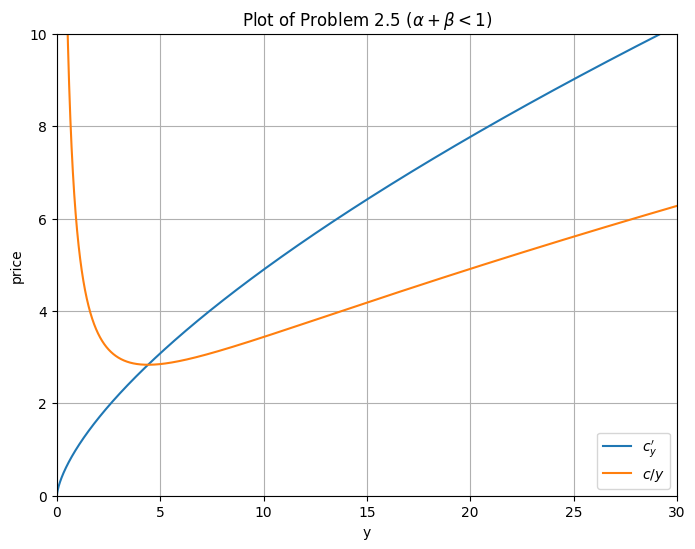
\includegraphics{/workspaces/TexFile/Microeconomic/graph/4.2.5.png}}
 \caption{$\alpha +\beta <1$}
 \label{fig:4.2.5}
\end{figure}

\item Let's compute the marginal cost \(c_{y}(w, r, s, y, \bar{F})\):

$$
\begin{aligned}
c_{y}(w, r, s, y, \bar{F}) &= \frac{y^{\frac{1-(\alpha+\beta)}{\alpha+\beta}}}{\alpha+\beta}\left(\frac{1}{A(\bar{F})^{\gamma}}\right)^{\frac{1}{\alpha+\beta}}\left[w\left(\frac{\beta}{\alpha} \frac{w}{r}\right)^{-\frac{\beta}{\alpha+\beta}}+r\left(\frac{\beta}{\alpha} \frac{w}{r}\right)^{\frac{\alpha}{\alpha+\beta}}\right] \\
&= \frac{y^{\frac{1-(1)}{1}}}{1}\left(\frac{1}{A(\bar{F})^{\gamma}}\right)^{\frac{1}{1}}\left[w\left(\frac{\beta}{\alpha} \frac{w}{r}\right)^{-\frac{\beta}{1}}+r\left(\frac{\beta}{\alpha} \frac{w}{r}\right)^{\frac{\alpha}{1}}\right] \\
&= y^0\left(\frac{1}{A(\bar{F})^{\gamma}}\right)\left[w\left(\frac{\beta}{\alpha} \frac{w}{r}\right)^{-\beta}+r\left(\frac{\beta}{\alpha} \frac{w}{r}\right)^{\alpha}\right] \\
&= \frac{1}{A(\bar{F})^{\gamma}}\left[w\left(\frac{\beta}{\alpha} \frac{w}{r}\right)^{-\beta}+r\left(\frac{\beta}{\alpha} \frac{w}{r}\right)^{\alpha}\right]
\end{aligned}
$$

The average variable cost (AVC) and the average cost (AC) are:


\begin{align}
    \begin{split}
        AVC &= \frac{wL^{*} + rK^{*}}{y} \\
&= \frac{w\left(\frac{y}{A(\bar{F})^{\gamma}}\right)^{\frac{1}{2}}\left(\frac{w\beta}{r}\right)^{-\
frac{\beta}{2}} + r\left(\frac{y}{A(\bar{F})^{\gamma}}\right)^{\frac{1}{2}}\left(\frac{w\beta}{r}\right)^{\frac{\beta}{2}}}{y} \\
&= \frac{w^{\frac{1}{2}}r^{\frac{1}{2}}}{y^{\frac{1}{2}}} \left(\frac{1}{A(\bar{F})^{\gamma}}\right)^{\frac{1}{2}} \left[w^{-\frac{\beta}{2}}y^{\frac{1}{2}} + r^{\frac{\beta}{2}}y^{\frac{1}{2}}\right] \\
&= \frac{w^{\frac{1}{2}}r^{\frac{1}{2}}}{y^{\frac{1}{2}}} \left(\frac{1}{A(\bar{F})^{\gamma}}\right)^{\frac{1}{2}} y^{\frac{1}{2}} \left[w^{-\frac{\beta}{2}} + r^{\frac{\beta}{2}}\right] \\
&= \frac{w^{\frac{1}{2}}r^{\frac{1}{2}}}{y^{\frac{1}{2}}} \left(\frac{1}{A(\bar{F})^{\gamma}}\right)^{\frac{1}{2}} \left[w^{-\frac{\beta}{2}} + r^{\frac{\beta}{2}}\right]  
    \end{split}
\end{align}



\begin{align}
    \begin{split}
        AC &= \frac{wL^{*} + rK^{*} + s\bar{F}}{y} \\
&= \frac{w\left(\frac{y}{A(\bar{F})^{\gamma}}\right)^{\frac{1}{2}}\left(\frac{w\beta}{r}\right)^{-\frac{\beta}{2}} + r\left(\frac{y}{A(\bar{F})^{\gamma}}\right)^{\frac{1}{2}}\left(\frac{w\beta}{r}\right)^{\frac{\beta}{2}} + s\bar{F}}{y} \\
&= \frac{w^{\frac{1}{2}}r^{\frac{1}{2}}}{y^{\frac{1}{2}}} \left(\frac{1}{A(\bar{F})^{\gamma}}\right)^{\frac{1}{2}} \left[w^{-\frac{\beta}{2}}y^{\frac{1}{2}} + r^{\frac{\beta}{2}}y^{\frac{1}{2}} + s\bar{F}y^{-\frac{1}{2}}\right] \\
&= \frac{w^{\frac{1}{2}}r^{\frac{1}{2}}}{y^{\frac{1}{2}}} \left(\frac{1}{A(\bar{F})^{\gamma}}\right)^{\frac{1}{2}} y^{\frac{1}{2}} \left[w^{-\frac{\beta}{2}} + r^{\frac{\beta}{2}} + s\bar{F}y^{-\frac{1}{2}}\right] \\
&= \frac{w^{\frac{1}{2}}r^{\frac{1}{2}}}{y^{\frac{1}{2}}} \left(\frac{1}{A(\bar{F})^{\gamma}}\right)^{\frac{1}{2}} \left[w^{-\frac{\beta}{2}} + r^{\frac{\beta}{2}} + s\bar{F}y^{-\frac{1}{2}}\right]
    \end{split}
\end{align}


The supply curve for the firm is the portion of the marginal cost curve that lies above the average variable cost curve. Mathematically, the supply curve is given by:

$$
p = y^{*}(w, r, s, \bar{F}) = \frac{1}{A(\bar{F})^{\gamma}}\left[w\left(\frac{\beta}{\alpha} \frac{w}{r}\right)^{-\beta}+r\left(\frac{\beta}{\alpha} \frac{w}{r}\right)^{\alpha}\right]
$$

The firm never wants to produce a positive and finite quantity of output despite constant returns to scale in labor and capital because the average variable cost (\(AVC\)) is always positive and increasing with output. When \(\alpha + \beta = 1\), the firm faces increasing returns to scale in labor and capital. This means that as the firm increases its output, the cost per unit of output decreases. However, the average variable cost (\(AVC\)) includes the fixed cost component (\(s\bar{F}\)) and, therefore, is not constant but increases with output. As a result, the firm would prefer not to produce any output rather than producing at a loss when the price is below the average variable cost, as the plot below shows :
\begin{figure}[H]
\centering
 \resizebox{0.75\textwidth}{!}{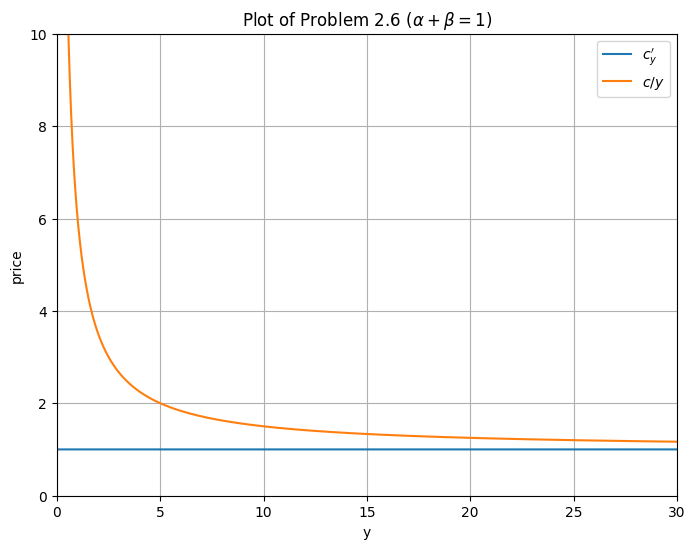
\includegraphics{/workspaces/TexFile/Microeconomic/graph/4.2.6.png}}
 \caption{$\alpha + \beta =1$}
 \label{}
\end{figure}

\item When $\alpha+\beta$ is greater than 1, both the marginal cost and average cost are falling as y increases, with the average cost consistently staying above the marginal cost. At any price p>0, the supply function becomes infinite. Refer to the graph for more clarity. Given that there are increasing returns to scale, the firm has an incentive to constantly increase production for better efficiency. This is not congruent with the principles of perfect competition, which necessitate firms to produce only a small quantity, as the plot below shows :
\begin{figure}[H]
\centering
 \resizebox{0.75\textwidth}{!}{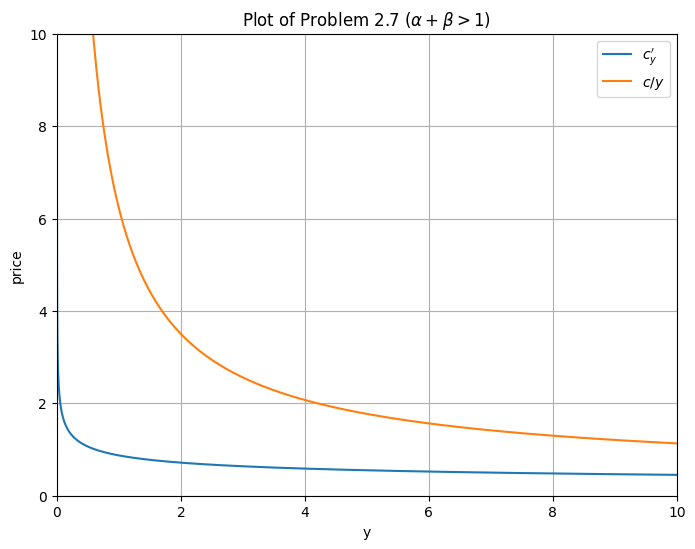
\includegraphics{/workspaces/TexFile/Microeconomic/graph/4.2.7.png}}
 \caption{}
 \label{}
\end{figure}

\item The overall market supply function, $Y^{S}$, is simply the cumulative sum of the J supply functions of individual firms, represented by:

\[Y^{S}=\sum_{j=1}^{J}\left[\frac{(\alpha+\beta) p}{D}\right]^{\frac{a+\beta}{1-(\alpha+\beta)}}=J\left[\frac{(\alpha+\beta) p}{D}\right]^{\frac{a+\beta}{1-(\alpha+\beta)}}\]

\item The aggregate market demand function, $Y^{D}$, is calculated by adding all the individual demand functions together:

\[Y^{D}=\sum_{j=1}^{J} y_{j}^{*}=\alpha \frac{\sum_{j=1}^{J} M_{j}}{p}\]

This overall demand function is not influenced by income distribution. This can be attributed to the fact that with Cobb-Douglas preferences, each consumer spends a fraction $\alpha$ of their income on mangoes.

\item The market-clearing price is found by equating demand $Y^{D}$ and supply $Y^{S}$, yielding:

\[Y^{S}=J\left[\frac{(\alpha+\beta) p_{M}}{D}\right]^{\frac{\alpha+\beta}{1-(\alpha+\beta)}}=\alpha \frac{\sum_{j=1}^{J} M_{j}}{p_{M}}=Y^{D}\]

which simplifies to:

\[p_{M}^{\frac{1}{1-(\alpha+\beta)}}=\alpha \frac{\sum_{j=1}^{J} M_{j}}{J}\left[\frac{(\alpha+\beta)}{D}\right]^{-\frac{\alpha+\beta}{1-(\alpha+\beta)}}\]

and further simplifies to:

\[p_{M} =\left[\alpha \frac{\sum_{j=1}^{J} M_{j}}{J}\right]^{1-(\alpha+\beta)}\left[\frac{(\alpha+\beta)}{D}\right]^{-(\alpha+\beta)}\]

Using equation in question 9, we derive:

\[Y =Y^{S}=Y^{D}=\alpha \sum_{j=1}^{J} M_{j}\left[\alpha \frac{\sum_{j=1}^{J} M_{j}}{J}\right]^{-(1-(\alpha+\beta))}\left[w\left(\frac{\beta}{\alpha} \frac{w}{r}\right)^{-\frac{\beta}{\alpha+\beta}}+r\left(\frac{\beta}{\alpha} \frac{w}{r}\right)^{\frac{\alpha}{\alpha+\beta}}\right]^{-(\alpha+\beta)}\]

\item The comparative statics are as follows:

(a) If total income $\sum_{j=1}^{J} M_{j}$ increases, both the equilibrium price and quantity produced rise. An increase in income corresponds to a positive demand shock, which raises demand and subsequently the price, considering the supply curve is upward sloping.

(b) An increase in productivity A lowers the equilibrium price while raising the quantity. A boost in productivity equates to a positive supply shock, which escalates demand and reduces the price, given the downward sloping demand curve. Consider the impact of increased productivity in computers: the quality of computers increases while the price drops.

\end{enumerate}
\end{document}